\section{Chapter 1 | D. Irga B. Naufal Fakhri D4 TI 2C}
\subsection{Sejarah Python}
	Python adalah bahasa pemrograman interpretatif multiguna dengan filosofi perancangan yang berfokus pada tingkat keterbacaan kode. Python diklaim sebagai bahasa yang menggabungkan kapabilitas, kemampuan, dengan sintaksis kode yang sangat jelas,dan dilengkapi dengan fungsionalitas pustaka standar yang besar serta komprehensif. 

	Python diciptakan oleh Guido van Rossum di Scitchting Mathematisch Centrum (CWI) di Belanda pada tahun 1990-an. Bahasa python terinspirasi dari bahasa pemrograman ABC dan merupakan kelanjutan dari bahasa tersebut. Nama python sendiri bukan berasal dari nama ular python namun karena Guido adalah penggemar grup komedi Inggris bernama Monty Python. Guido masih menjadi penulis utama untuk python, walaupun python bersifat open source sehingga ribuan orang juga berkontribusi dalam mengembangkan python.

	Di tahun 1995, Guido melanjutkan pembuatan python di Corporation for National Research Initiative (CNRI) di Virginia Amerika, dimana dia merilis beberapa versi dari python.
Pada Mei 2000, Guido dan tim Python pindah ke BeOpen.com dan membentuk tim BeOpen PythonLabs. Di bulan Oktober pada tahun yang sama, tim python pindah ke Digital Creation (sekarang menjadi Perusahaan Zope). Pada tahun 2001, dibentuklah Organisasi Python yaitu Python Software Foundation (PSF). PSF merupakan organisasi nirlaba yang dibuat khusus untuk semua hal yang berkaitan dengan hak intelektual Python. Perusahaan Zope menjadi anggota sponsor dari PSF.

\subsection{Tanggal Rilis Python}
Semua versi python yang dirilis bersifat open source. Dalam sejarahnya, hampir semua rilis python menggunakan lisensi GFL-compatible. Berikut adalah versi major dan minor python berikut tanggal rilisnya.
\begin{itemize}
  \item Python 1.0 – Januari 1994
  \item Python 1.2 – 10 April 1995
  \item Python 1.3 – 12 Oktober 1995
  \item Python 1.4 – 25 Oktober 1996
  \item Python 1.5 – 31 Desember 1997
  \item Python 1.6 – 5 September 2000
  \item Python 2.0 – 16 Oktober 2000
  \item Python 2.1 – 17 April 2001
  \item Python 2.2 – 21 Desember 2001
  \item Python 2.3 – 29 Juli 2003
  \item Python 2.4 – 30 Nopember 2004
  \item Python 2.5 – 19 September 2006
  \item Python 2.6 – 1 Oktober 2008
  \item Python 2.7 – 3 Juli 2010
  \item Python 3.0 – 3 Desember 2008
  \item Python 3.1 – 27 Juni 2009
  \item Python 3.2 – 20 Februari 2011
  \item Python 3.3 – 29 September 2012
  \item Python 3.4 – 16 Maret 2014
  \item Python 3.5 – 13 September 2015
  \item Python 3.6 – 23 Desember 2016
\end{itemize}

\subsection{Perbedaan Python 2 dengan Python 3}
Pada Python 2 dan Python 3 memiliki kesamaan kapabilitas namun cara penggunaannya berbeda
\begin{itemize}
\item Print
\end{itemize}
Pada python2, print lebih seperti statement daripada fungsi
\begin{lstlisting}
print "Saya Belajar Python"
\end{lstlisting}
sedangkan pada python3, print digunakan sebagai fungsi
\begin{lstlisting}
print("Saya Belajar Python")
\end{lstlisting}

\begin{itemize}
\item Pembagian pada Interger
\end{itemize}
Pada Python 2, semua tipe data angka yang tidak mengandung desimal akan diperlakukan sebagai integer. Terlihat mudah pada awalnya, ketika mencoba untuk membagi kedua integer akan didapatkan tipe data float.

\begin{lstlisting}
3 / 2 = 1.5
\end{lstlisting}

Python 2 menggunakan floor division atau dibulatkan ke nilai paling rendah misalnya 1.5 jadi 1, 2.6 jadi 2 dan seterusnya. Pada Python 2.7 akan menjadi seperti ini:

\begin{lstlisting}
3
4
x = 3 / 2
print a
#Output
1
\end{lstlisting}

Untuk desimal maka tambahkan .0 setelah bilangan dan menjadi seperti ini 3.0 / 2.0  untuk mendapatkan hasil 1.5
Pada Python 3, pembagian pada bilangan integer lebih intuitif:

\begin{lstlisting}
a = 3 / 2
print(a)
#Output
1.5
\end{lstlisting}

Kita juga masih bisa melakukan 3.0 / 2.0  untuk mendapatkan 1.5 namun untuk mendapatkan floor division maka pada Python 3 gunakan //:
\begin{lstlisting}
b = 3 // 2
print(b)
#Output
1
\end{lstlisting}
Fitur pada Python 3 ini tidak bisa digunakan pada Python 2.7

\begin{itemize}
\item Dukungan Unicode
\end{itemize}

Ketika bahasa pemrograman menangani tipe data string (yang mana merupakan sekumpulan karakter), mereka bisa melakukan beberapa cara berbeda sehingga komputer dapat mengubah angka ke huruf dan simbol lain. Python 2 menggunakan alfabet ASCII secara default, sehingga ketika kita mengetik "Halo!"  maka Python 2 menangani string sebagai ASCII. Terbatas pada beberapa ratus karakter, ASCII mungkin bukan pilihan yang fleksibel untuk menangani proses encoding terutama yang non English.

Untuk menggunakan unicode yang lebih luwes, mendukung lebih dari 128,000 karakter maka kita harus mengetik u"Halo!" , dengan tambahan u  di depannya yang mana berarti Unicode.

Python 3 menggunakan Unicode secara default, yang mana menyelamatkan programmer dari tambahan kode lagi, lebih hemat waktu dan mudah untuk diisikan dan ditampilkan. Karena Unicode mendukung berbagai karakter linguistik yang beragam termasuk menampilkan emoji, penggunaan karakter secara default dengan encoding memastikan perangkat mobile didukung oleh program yang kita buat.

Jika kita ingin kode Python 3 kita mendukung Python 2, tambahkan u di depan string.

\subsection{Penggunaan Python di perusahaan dunia}
\begin{enumerate}
  \item Google adalah perusahaan besar yang menggunakan banyak kode Python di dalam mesin pencarinya. Dan mesin pencari google adalah yang paling terkenal di dunia.
  \item Youtube, situs video terbesar dan terpopuler di dunia, sebagian besar kodenya ditulis dalam bahasa Python.
  \item Facebook, media sosial terbesar di dunia, menggunakan Tornado, sebuah framework Python untuk menampilkan timeline.
  \item Instagram, siapa yang tidak kenal. Instagram menggunakan Django, framework python sebagai mesin pengolah sisi server dari aplikasinya.
  \item Pinterest, banyak menggunakan python untuk membangun aplikasinya.
  \item Dropbox, barangkali Anda adalah salah seorang pengguna layanan ini. Dropbox menggunakan python baik di sisi server maupun di sisi pengguna layanannya.
  \item Quora, salah satu situs tanya jawab terbesar di dunia, dibangun menggunakan Python.
  \item NASA, badan antariksa Amerika ini menggunakan Python untuk bidang sainsnya.
  \item NSA, badan mata – mata Amerika banyak menggunakan Python untuk analisa kriptografi dan intelijen
  \item Blender, Maya, software pembuat animasi 3D terkenal, menggunakan Python sebagai salah satu bahasa skrip pemrogramannya.
  \item Raspberry Pi, komputer mini yang banyak digunakan sebagai mikrokontroller, menggunakan Python sebagai bahasa utamanya.
  \item ESRI, produsen terkenal pembuat software pemetaan GIS banyak menggunakan Python di produknya.
\end{enumerate}
Untuk lebih lengkapnya bisa mengunjungi www.python.org/about/success/



\subsection{Cara menginstall Anaconda}
\begin{enumerate}
  \item Pastikan anda telah menginstall python dan anda mengetahui versi dari python yang telah anda install
  \item Download Anaconda dari website www.anaconda.com/distribution
  \item pilih sesuai dengan versi python anda, jika versi anda python3 maka pilih python3
  \item Setelah itu buka file yang telah anda download
  \item Setelah muncul gambar dibawah ini, tekan next
\begin{figure}[!htbp]
  \centering
  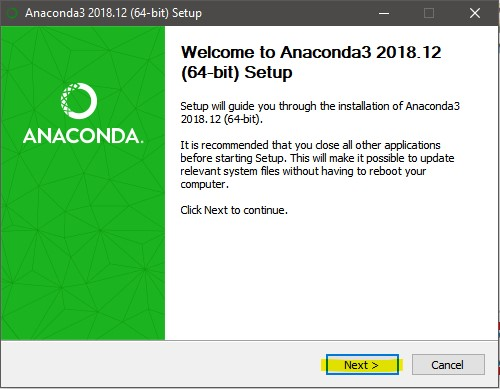
\includegraphics[height=3cm]{chapters/gambar/install1.jpg}
  \caption{Tampilan Instalasi 1}
\end{figure}

  \item Baca license agreement lalu tekan 'I Agree'
\begin{figure}[!htbp]
  \centering
  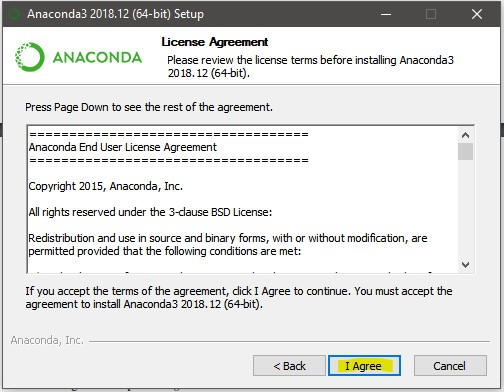
\includegraphics[height=3cm]{chapters/gambar/install2.jpg}
  \caption{Tampilan Instalasi 2}
\end{figure}

  \item Setelah itu pilih mau diinstall pada user yang sedang anda pakai atau kesemua user, direkomendasikan untuk memilih just me yaitu hanya user yang sedang dipakai saja
\begin{figure}[!htbp]
  \centering
  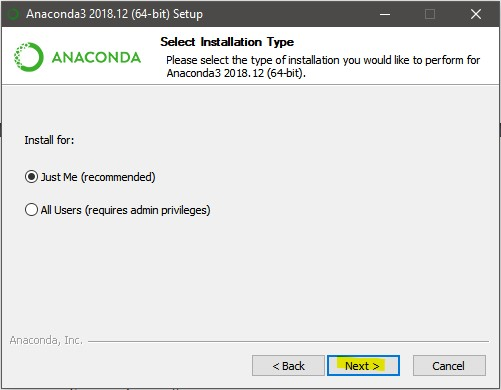
\includegraphics[height=3cm]{chapters/gambar/install3.jpg}
  \caption{Tampilan Instalasi 3}
\end{figure}

  \item Catat tempat dimana anda akan menginstall anaconda, lalu tekan 'Next'
\begin{figure}[!htbp]
  \centering
  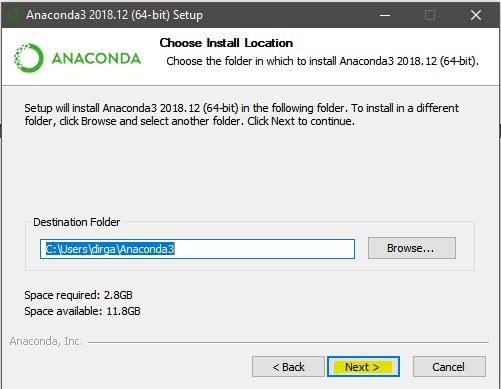
\includegraphics[height=3cm]{chapters/gambar/install4.jpg}
  \caption{Tampilan Instalasi 4}
\end{figure}

  \item Setelah itu anda diberi pilihan, direkomendasikan untuk tidak mengubah pilihan tersebut, lalu tekan 'Install'
\begin{figure}[!htbp]
  \centering
  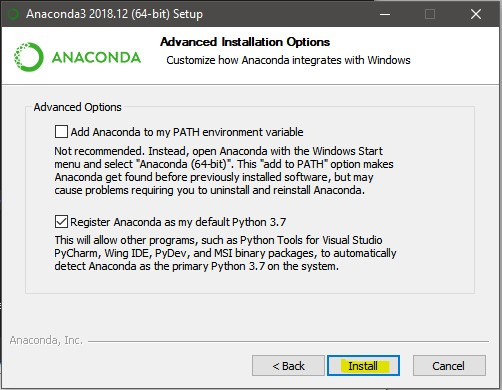
\includegraphics[height=3cm]{chapters/gambar/install5.jpg}
  \caption{Tampilan Instalasi 5}
\end{figure}

  \item Tunggu sampai instalasi selesai
\begin{figure}[!htbp]
  \centering
  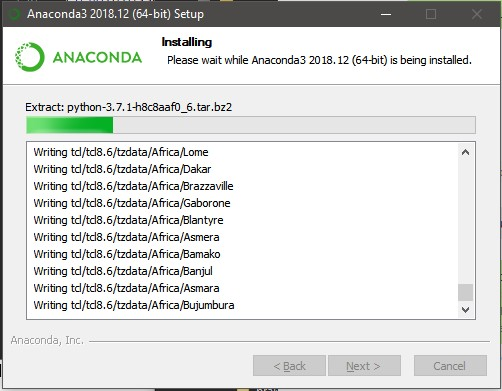
\includegraphics[height=3cm]{chapters/gambar/install6.jpg}
  \caption{Tampilan Instalasi 6}
\end{figure}

  \item Setelah selesai tekan 'Next'
\begin{figure}[!htbp]
  \centering
  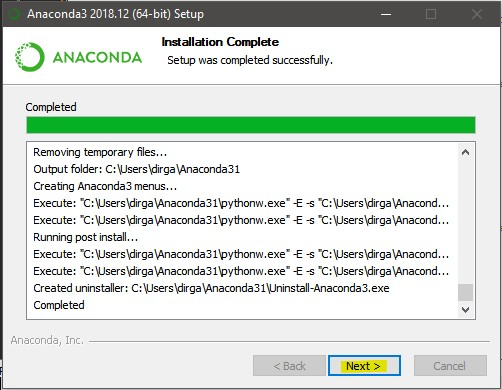
\includegraphics[height=3cm]{chapters/gambar/install7.jpg}
  \caption{Tampilan Instalasi 7}
\end{figure}

  \item Setelah itu ada opsi untuk memilih untuk meinstall visual studio code, jika anda berminat klik 'Install VSCode' jika tidak tekan 'Skip'
\begin{figure}[!htbp]
  \centering
  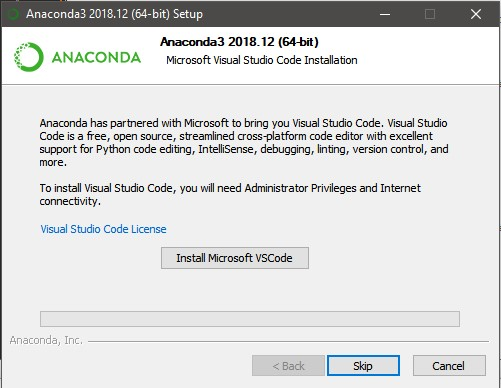
\includegraphics[height=3cm]{chapters/gambar/install8.jpg}
  \caption{Tampilan Instalasi 8}
\end{figure}

  \item Tekan 'Finish' untuk menyelesaikan instalasi
\begin{figure}[!htbp]
  \centering
  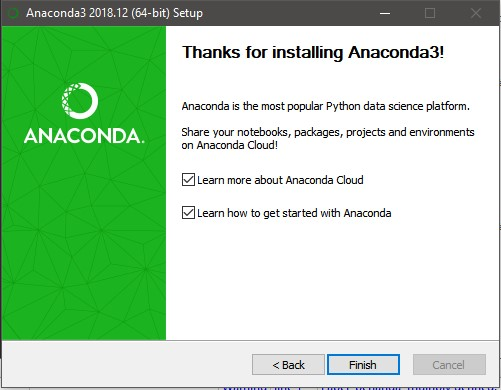
\includegraphics[height=3cm]{chapters/gambar/install9.jpg}
  \caption{Tampilan Instalasi 9}
\end{figure}

\end{enumerate}

\subsection{Cara menggunakan Spyder pada Anaconda}
Pertama buka aplikasi Anaconda sampai muncul seperti ini
\begin{figure}[!htbp]
  \centering
  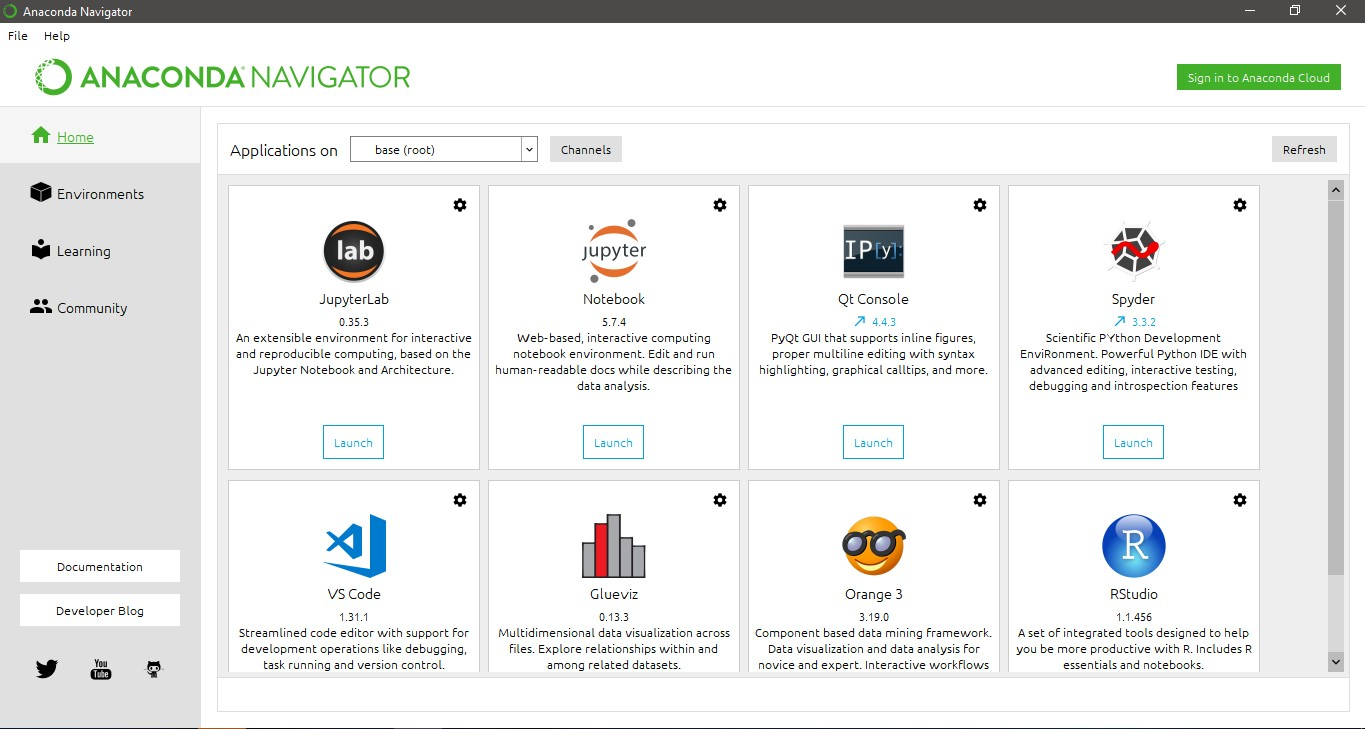
\includegraphics[height=3cm]{chapters/gambar/gambaranaconda.jpg}
  \caption{Tampilan awal Anaconda}
\end{figure}

Setelah itu tekan Launch dibawah logo Spyder
Tunggu sampai muncul seperti ini
\begin{figure}[!htbp]
  \centering
  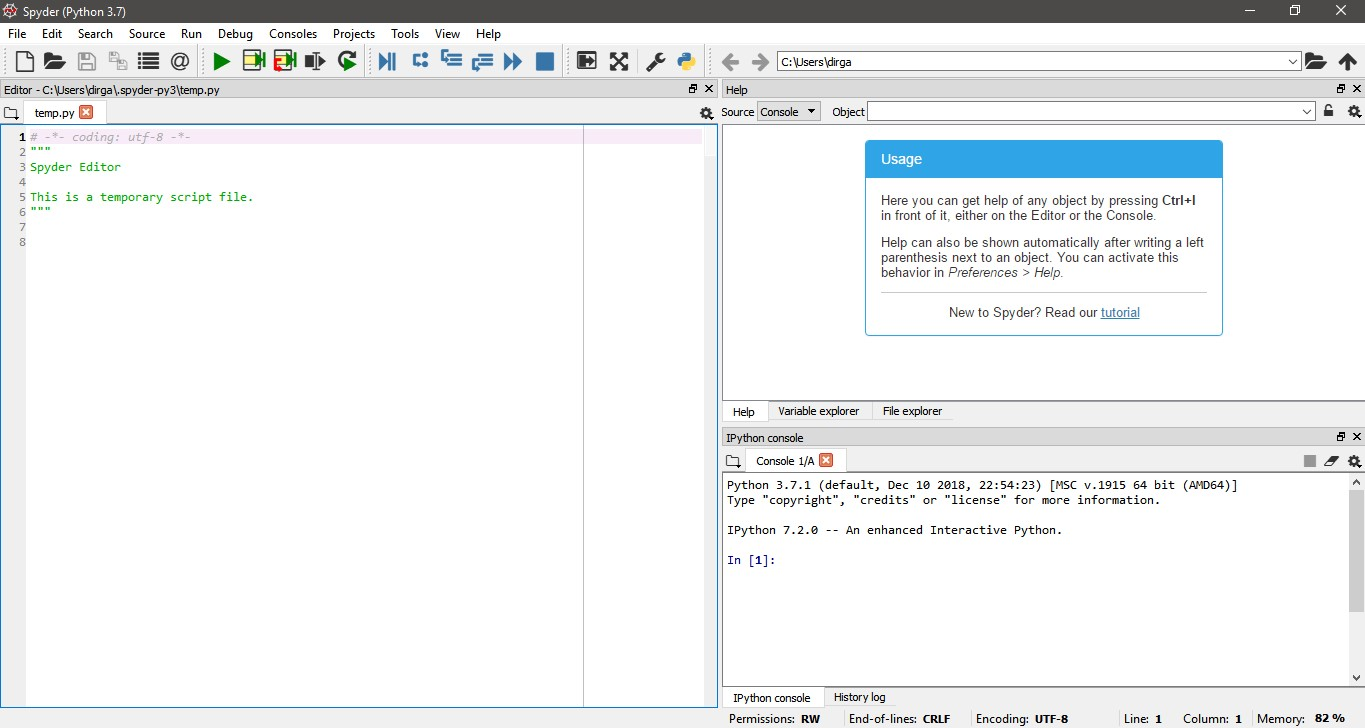
\includegraphics[height=3cm]{chapters/gambar/gambarspider.jpg}
  \caption{Tampilan spider}
\end{figure}

\subsection{Membuat Hello World di Spyder}
Setelah membuka spyder seperti gambar di section sebelumnya tekan menu File lalu klik New File atau bisa menggunakan kombinasi tombol Ctrl + N sampai muncul seperti ini

\begin{figure}[!htbp]
  \centering
  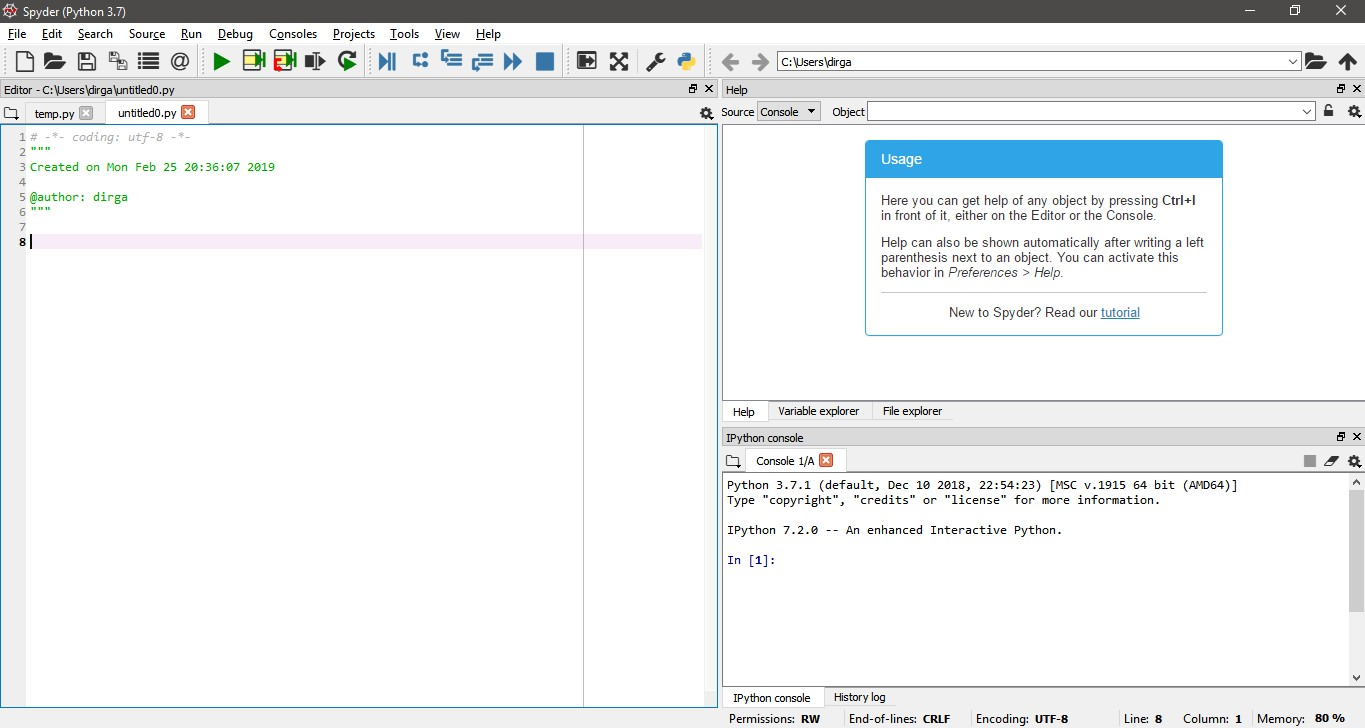
\includegraphics[height=3cm]{chapters/gambar/gambarnewfile.jpg}
  \caption{Tampilan new file pada spider}
\end{figure}

Karena kita menggunakan Python3.7 maka kita menggunakan funsi print() untuk memunculkan teks Hello World yang akan kita buat, tuliskan print("Hello World") pada teks editor di Spyder

\begin{figure}[!htbp]
  \centering
  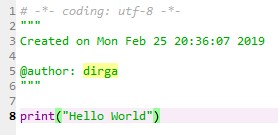
\includegraphics[height=3cm]{chapters/gambar/gambarprint.jpg}
  \caption{print("Hello World")}
\end{figure}

setelah itu tekan tombol play berwarna hijau diatas, karena kita belum save file yang kita buat maka akan muncul dialog simpan file, pilih tempat dan nama file yang akan disimpan contohnya helloworld.py

\begin{figure}[!htbp]
  \centering
  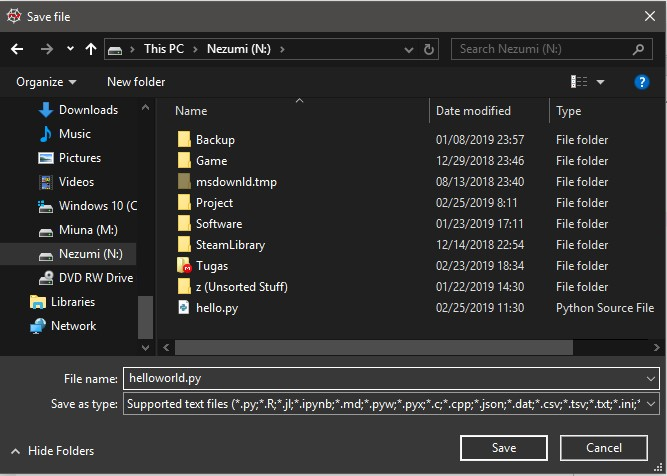
\includegraphics[height=3cm]{chapters/gambar/helloworld.jpg}
  \caption{Dialog simpan file}
\end{figure}

setelah itu tekan run maka hasil dari program yang kita buat tadi ada dibagian console yang berada di pinggir kanan bawah

\begin{figure}[!htbp]
  \centering
  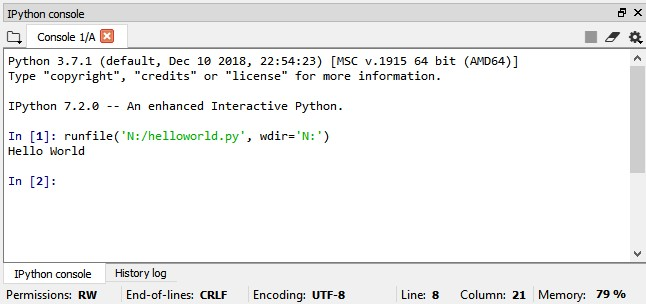
\includegraphics[height=3cm]{chapters/gambar/hasil.jpg}
  \caption{Hasil Program}
\end{figure}

